\documentclass[12pt, a4paper]{article}
\usepackage{../../../myconfig} % Gọi file cấu hình từ ngoài gốc vào

% ==========================================
% BẮT ĐẦU NỘI DUNG TÀI LIỆU
% ==========================================
\begin{document}

% Truyền 3 tham số: {Nhãn cam} {Chữ to chính giữa} {Chữ ở góc phải Header}
\titlebox{Chủ đề: Hàm số}{Giá trị lớn nhất - giá trị nhỏ nhất}{Hàm số: GTLN - GTNN}
\drawdashlines{29}
\newpage

% --- CÂU 1: ĐỒ THỊ HÀM SỐ TRÊN ĐOẠN [-3;5] ---
\questionLinesManual{5}{1}{ Cho hàm số \( y = f(x) \) liên tục trên đoạn \([-3; 5]\) và có đồ thị như hình vẽ. Giá trị lớn nhất của hàm số \( y = f(x) \) trên đoạn \([-3; 5]\) bằng

\begin{center}
\begin{tikzpicture}[>=latex, scale=0.8]
    % 1. Vẽ hệ trục tọa độ Ox, O
    \draw[->] (-4,0) -- (5.5,0) node[below] {\small $x$};
    \draw[->] (0,-3) -- (0,4.5) node[right] {\small $y$};
    \node[below left] at (0,0) {\small $O$};
    
    % 2. Vẽ đồ thị hàm số (dạng sóng)
    \draw[thick, color=black!80, samples=150, domain=-3:1] 
       plot (\x, {\x + 1});
    \draw[thick, color=black!80, samples=150, domain=1:5]    
        plot (\x, {3/8*\x*\x - 2*\x + 29/8});   
    % 3. Đánh dấu các điểm
    \draw[dashed] (0,-2) -- (-3,-2) -- (-3,0);
    \draw[dashed] (3,0) -- (3,1) -- (0,1);
     \draw[dashed] (1,0) -- (1,2) -- (0,2);
    \draw[dashed] (5,0) -- (5,3) -- (0,3);
    \node[below] at (-3,0) {\small $-3$};
    \node[below] at (5,0) {\small $5$};
    \node[left] at (0,3) {\small $3$};
    \node[left] at (0,2) {\small $2$};
    \node[left] at (0,1) {\small $1$};
    \node[right] at (0,-2) {\small $-2$};
    \node[below] at (-1,0) {\small $-1$};
    \node[below] at (1,0) {\small $1$};
    \node[below] at (3,0) {\small $3$};
\end{tikzpicture}
\end{center}
}

\questionLinesManual{5}{2}{ Cho hàm số \( y = f(x) \) liên tục và có đồ thị trên đoạn \([-2; 4]\) như hình vẽ bên. Tổng giá trị lớn nhất và nhỏ nhất của hàm số \( y = f(x) \) trên đoạn \([-2; 4]\) bằng

\begin{center}
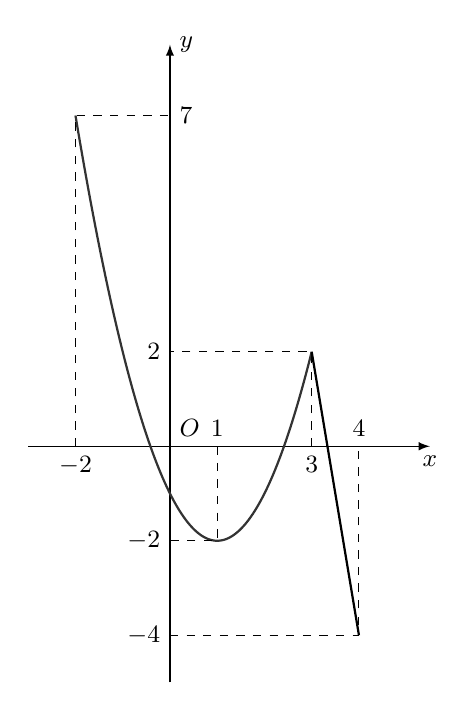
\begin{tikzpicture}[>=latex, scale=0.6]
    % 1. Vẽ hệ trục tọa độ Ox, Oy
    \draw[->] (-3,0) -- (5.5,0) node[below] {\small $x$};
    \draw[->] (0,-5) -- (0,8.5) node[right] {\small $y$};
    \node[above right] at (0,0) {\small $O$};
    
    % 2. Vẽ đồ thị hàm số (dạng đa thức bậc 3)
    \draw[thick, color=black!80, samples=150, domain=-2:3] 
        plot (\x, {\x*\x - 2*\x - 1});
    \draw[thick] (3,2) -- (4,-4);
    % 3. Đánh dấu các điểm
    \draw[dashed] (0,-4) -- (4,-4) -- (4,0);
    \draw[dashed] (1,0) -- (1,-2) -- (0,-2);
    \draw[dashed] (3,0) -- (3,2) -- (0,2);
    \draw[dashed] ( -2,0) -- (-2,7) -- (0,7);
    \node[above] at (4,0) {\small $4$};
    \node[left] at (0,-4) {\small $-4$};
    \node[right] at (0,7) {\small $7$};
    \node[left] at (0,-2) {\small $-2$};
    \node[left] at (0,2) {\small $2$};
    % Đánh dấu các mốc trên trục Ox
    \node[below] at (-2,0) {\small $-2$};
    \node[above] at (1,0) {\small $1$};
    \node[below] at (3,0) {\small $3$};
\end{tikzpicture}
\end{center}
}

\questionLinesManual{5}{3}{ Cho hàm số \( y = f(x) \) liên tục trên đoạn \([1; 5]\) và có đồ thị trên như hình vẽ sau.

\begin{center}
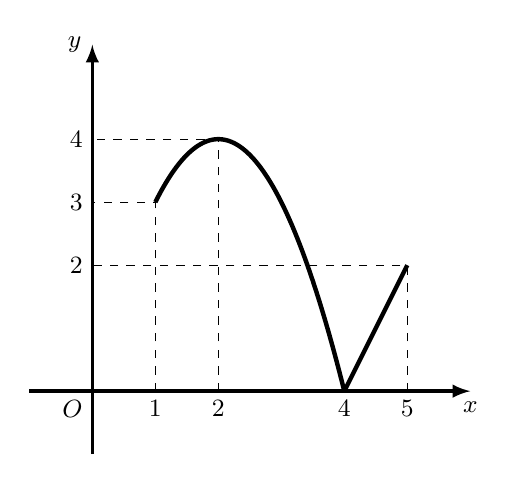
\begin{tikzpicture}[>=latex, scale=0.8]
    % 1. Hệ trục tọa độ Ox, Oy dày và rõ nét
    \draw[->, line width=1.2pt] (-1,0) -- (6,0) node[below] {\small $x$};
    \draw[->, line width=1.2pt] (0,-1) -- (0,5.5) node[left] {\small $y$};
    \node[below left] at (0,0) {\small $O$};
    
    % 2. Đồ thị hàm số từng nhánh
    % Nhánh 1: Parabol từ x = 1 (y = 3) đạt cực đại tại đỉnh x = 2 (y = 4) xuôi xuống x = 4 (y = 0)
    % Hàm phù hợp: y = -(x-2)^2 + 4
    \draw[ultra thick, samples=150, domain=1:4] plot (\x, {-(\x-2)*(\x-2) + 4});
    % Nhánh 2: Đoạn thẳng từ (4, 0) lên (5, 2)
    \draw[ultra thick] (4,0) -- (5,2);

    % 3. Đường nét đứt và điền số trục tọa độ
    % Tại x = 1, y = 3
    \draw[dashed] (1,0) -- (1,3) -- (0,3);
    \node[below] at (1,0) {\small $1$};
    \node[left] at (0,3) {\small $3$};
    
    % Tại x = 2, y = 4 (Đỉnh)
    \draw[dashed] (2,0) -- (2,4) -- (0,4);
    \node[below] at (2,0) {\small $2$};
    \node[left] at (0,4) {\small $4$};
    
    % Tại x = 4, y = 0
    \node[below] at (4,0) {\small $4$};
    
    % Tại x = 5, y = 2
    \draw[dashed] (5,0) -- (5,2) -- (0,2);
    \node[below] at (5,0) {\small $5$};
    \node[left] at (0,2) {\small $2$};

\end{tikzpicture}
\end{center}

Trên đoạn \([1; 5]\), hàm số đã cho đạt giá trị lớn nhất tại điểm}

\questionLinesManual{5}{4}{ Cho hàm số \( f(x) \) liên tục trên \([-1; 5]\) và có đồ thị trên đoạn \([-1; 5]\) như hình vẽ bên dưới. Tổng giá trị lớn nhất và giá trị nhỏ nhất của hàm số \( f(x) \) trên đoạn \([-1; 5]\) bằng

\begin{center}
\begin{tikzpicture}[>=latex, scale=0.8]
    % 1. Hệ trục tọa độ Ox, Oy
    \draw[->] (-2,0) -- (6,0) node[below] {\small $x$};
    \draw[->] (0,-3) -- (0,4) node[right] {\small $y$};
    \node[below left] at (0,0) {\small $0$};
    
    % 2. Đồ thị hàm số (vẽ bằng lệnh plot trơn tru qua các điểm cực trị)
    % Các điểm uốn và cực trị: (-1, -2), (0, 1) [Cực đại], (2, -2) [Cực tiểu], (4.25, 3) [Cực đại], (5, 1)
    \draw[thick,samples=150, domain=-1:5]
plot (\x, {-0.1588135590717*\x*\x*\x*\x + 1.2862146877635*\x*\x*\x - 2.3097740105484*\x*\x - 0.7548022573836*\x + 1});    % 3. Đường nét đứt và điền số trục tọa độ
    % Tại x = -1, y = -2
    \draw[dashed] (-1,0) -- (-1,-2) -- (0,-2);
    \node[above] at (-1,0) {\small $-1$};
    \node[below left] at (0,-2) {\small $-2$};
    
    % Tại x = 0, y = 1
    \node[above left] at (0,1) {\small $1$};
    
    % Tại x = 2, y = -2
    \draw[dashed] (2,0) -- (2,-2);
    \node[above] at (2,0) {\small $2$};
    
    % Tại đỉnh cực đại thứ hai (x ≈ 4.25, y = 3)
    \draw[dashed] (4.25,0) -- (4.25,3) -- (0,3);
    \node[left] at (0,3) {\small $3$};
    
    % Tại điểm cuối cùng x = 5, y = 1
    \draw[dashed] (5,0) -- (5,1) -- (0,1);
    \node[below] at (5,0) {\small $5$};

\end{tikzpicture}
\end{center}}

\newpage
\drawdashlines{35}
\newpage

\questionLinesManual{10}{5}{ Tìm giá trị nhỏ nhất của hàm số \( f(x) = x^4 - 2x^2 - 1 \). }

\questionLinesManual{10}{6}{ Tìm giá trị lớn nhất của hàm số \( f(x) = -x^2 +2x- 1 \). }

\questionLinesManual{10}{7}{ Giá trị lớn nhất của hàm số \( f(x) = x^3 - 3x^2 - 9x + 10 \) trên đoạn \([-2; 2]\) bằng:}

\questionLinesManual{10}{8}{ Giá trị nhỏ nhất của hàm số \( f(x) = x^3 - 3x + 2 \) trên đoạn \([-3; 3]\) bằng}

\questionLinesManual{8}{9}{ Giá trị lớn nhất của hàm số \( f(x) = -x^4 + 12x^2 + 1 \) trên đoạn \([-1; 2]\) bằng}

\questionLinesManual{8}{10}{ Giá trị nhỏ nhất của hàm số \( f(x) = x^3 - 6x^2 + 9x - 1 \) trên nửa khoảng \([-1; +\infty)\) là}

\questionLinesManual{8}{11}{ Tìm giá trị nhỏ nhất của hàm số \( y = -x + 3 - \dfrac{1}{x + 2} \) trên nửa khoảng \([-4; -2)\).}

\questionLinesManual{8}{12}{Tìm tập giá trị của hàm số \( y = \sqrt{x - 1} + \sqrt{9 - x} \)}

\questionLinesManual{8}{13}{ Gọi \( M, m \) lần lượt là giá trị lớn nhất và giá trị nhỏ nhất của hàm số \( y = 2 - \sin x \). Khẳng định nào sau đây đúng?}

\questionLinesManual{8}{14}{Gọi \( m \) là giá trị nhỏ nhất của hàm số \( y = x - 1 + \dfrac{4}{x - 1} \) trên khoảng \( (1; +\infty) \). Tìm \( m \)?}

\questionLinesManual{8}{15}{ Giá trị nhỏ nhất của hàm số \( y = x - 5 + \dfrac{1}{x} \) trên khoảng \( (0; +\infty) \) bằng bao nhiêu?}

\questionLinesManual{5}{16}{Cho hàm số \( y = f(x) \) liên tục trên đoạn \([-4; 4]\) có bảng biến thiên như hình vẽ

\begin{center}

\begin{tikzpicture}[>=stealth]
    % Khởi tạo bảng biến thiên với độ rộng cột tiêu đề và khoảng cách giữa các số
    \tkzTabInit[nocadre=false, lgt=1.2, espcl=3]
        {$x$ / 1, $y'$ / 1, $y$ / 2.5}     % Tên các dòng và chiều cao dòng
        {$-4$, $-1$, $3$, $4$}             % Các giá trị trên dòng x
    
    % Xét dấu của đạo hàm y'
    \tkzTabLine{ , +, 0, -, 0, + }
    
    % Sự biến thiên của hàm số y (mũi tên đi lên/xuống)
    \tkzTabVar{-/ $-71$, +/ $10$, -/ $-22$, +/ $-15$}
\end{tikzpicture}
\end{center}

Giá trị nhỏ nhất của hàm số đã cho trên đoạn \([-4; 4]\) bằng}

\questionLinesManual{5}{17}{ Cho hàm số \( y = f(x) \) liên tục và có bảng biến thiên trên đoạn \([-1; 3]\) như hình vẽ bên. Khẳng định nào sau đây là đúng?

\begin{center}

\begin{tikzpicture}[>=stealth]
    % Khởi tạo bảng biến thiên với độ rộng cột tiêu đề và khoảng cách giữa các số
    \tkzTabInit[nocadre=false, lgt=1.2, espcl=3]
        {$x$ / 1, $y'$ / 1, $y$ / 2.5}     % Tên các dòng và chiều cao dòng
        {$-1$, $0$, $2$, $3$}              % Các giá trị trên dòng x
    
    % Điền các dấu và giá trị 0 của đạo hàm y'
    \tkzTabLine{ , +, 0, -, 0, + }
    
    % Điền các mũi tên biến thiên và giá trị cực trị của hàm số y
    \tkzTabVar{-/ $0$, +/ $5$, -/ $1$, +/ $4$}
\end{tikzpicture}
\end{center}

}{
    \begin{tasks}(4)
        \task \( \max\limits_{[-1;3]} f(x) = 4 \)
        \task \( \max\limits_{[-1;3]} f(x) = 5 \)
        \task \( \max\limits_{[-1;3]} f(x) = 1 \)
        \task \( \max\limits_{[-1;3]} f(x) = 0 \)
    \end{tasks}
}

\questionLinesManual{5}{18}{ Cho hàm số \( y = f(x) \) có bảng xét dấu đạo hàm như sau

\begin{center}

\begin{tikzpicture}[>=stealth]
    % Khởi tạo bảng xét dấu gồm 2 dòng: x và y'
    \tkzTabInit[nocadre=false, lgt=1.2, espcl=2.5]
        {$x$ / 1, $y'$ / 1}                               % Tên dòng / Chiều cao dòng
        {$-\infty$, $-1$, $0$, $1$, $+\infty$}            % Các giá trị trên dòng x
    
    % Xét dấu của đạo hàm y', sử dụng 'd' để tạo dấu hai gạch || tại x = -1
    \tkzTabLine{ , -, d, -, 0, +, 0, - }
\end{tikzpicture}
\end{center}

Mệnh đề nào sau đây đúng?}{
    \begin{tasks}(4)
        \task \(\max\limits_{(0;+\infty)} f(x) = f(1)\)
        \task \(\max\limits_{[-1;1]} f(x) = f(0)\)
        \task \(\max\limits_{(-\infty;-1]} f(x) = f(-1)\)
        \task \(\min\limits_{(0;1]} f(x) = f(0)\)
    \end{tasks}
}

% --- CÂU 4 ---
\questionShortAnswer{10}{19}{Trong 5 giây đầu tiên, một chất điểm chuyển động theo phương trình \( s(t) = t^3 - 3t^2 + 8t + 2 \). Trong đó, \( t \) tính bằng giây và \( s \) tính bằng mét. Chất điểm có vận tốc tức thời nhỏ nhất bằng bao nhiêu \( m/s \) trong 5 giây đầu tiên đó?}

% --- CÂU 8 ---
\questionShortAnswer{10}{20}{Một chất điểm chuyển động theo qui luật \( s = 6t^2 - t^3 \) (trong đó \( t \) là khoảng thời gian tính bằng giây mà chất điểm bắt đầu chuyển động). Tính thời điểm \( t \) (giây) mà tại đó vận tốc (m/s) của chuyển động đạt giá trị lớn nhất.}

% --- CÂU 9 ---
\questionShortAnswer{10}{21}{Bạn Minh ngồi trên máy bay đi du lịch thế giới với vận tốc chuyển động của máy bay là  
\[v(t) = -t^2 +20t+100  \, (\text{m/s}).\]
Vận tốc lớn nhất máy bay đạt được là bao nhiêu:}

% --- CÂU 5 ---
\questionShortAnswer{10}{22}{Ngày khai giảng năm học 2026 – 2027, học sinh khối 12 trường THPT Thanh Miện thả chùm bóng bay gắn thông điệp "Học Sinh khối 12 chiến thắng CT2018". Ước tính độ cao \( h \) (tính bằng km) của chùm bóng bay so với mặt đất vào thời điểm \( t \) (đơn vị giờ) được cho bởi công thức  
\[h(t) = -t^3 + 3t^2 \quad (0 \leq t \leq 3).\]  
Chùm bóng bay đạt độ cao lớn nhất so với mặt đất là \( a \, (km) \). Tìm \( a \).}

% --- CÂU 6 ---
\questionShortAnswer{10}{23}{Sau khi phát hiện ra dịch bệnh vi rút Đậu mùa Khỉ, các chuyên gia y tế ước tính số người nhiễm bệnh kể từ khi xuất hiện bệnh nhân đầu tiên đến ngày thứ \( x \) là \( f(x) = -x^3 + 18x^2 \). Ta xem \( f'(x) \) là tốc độ truyền bệnh tại thời điểm \( x \). Tốc độ truyền bệnh sẽ lớn nhất vào ngày thứ bao nhiêu?}

% --- CÂU 7 ---
\questionShortAnswer{10}{24}{Một doanh nghiệp dự định sản xuất không quá 500 sản phẩm. Nếu doanh nghiệp sản xuất \( x \) sản phẩm (\( 1 \leq x \leq 500 \)) thì doanh thu nhận được khi bán hết số sản phẩm đó là  
\( F(x) = x^3 - 1999x^2 + 1001000x + 250000 \)  
(đồng), trong khi chi phí sản xuất bình quân cho một sản phẩm là  
\( G(x) = x + 1000 + \dfrac{250000}{x} \) 
(đồng). Doanh nghiệp cần sản xuất bao nhiêu sản phẩm để lợi nhuận thu được là lớn nhất?}

\end{document}